\documentclass[conference]{IEEEtran}
\usepackage{graphicx}
\usepackage[utf8]{inputenc}
\usepackage[T5]{fontenc}
\usepackage[vietnamese]{babel}
\usepackage{amsmath}
\usepackage{hyperref}
\usepackage{caption}
\usepackage{subcaption}
\usepackage{booktabs}
\usepackage{float}
\usepackage{url}


\title{Ứng dụng AI và IoT trong Phân Tích và Điều Chỉnh Tư Thế Ngồi}

% === Tác giả ===
\author{
    \textbf{Đặng Thanh Bình, Tạ Việt Anh, Vũ Hải Đức, Nguyễn Tuấn Anh} \\
    \textit{Nhóm 5, CNTT 16-04, Khoa Công Nghệ Thông Tin} \\
    \textit{Trường Đại Học Đại Nam, Việt Nam} \\
    \textbf{ThS. Nguyễn Văn Nhân, ThS. Lê Trung Hiếu} \\
    \textit{Giảng viên hướng dẫn, Khoa Công Nghệ Thông Tin} \\
    \textit{Trường Đại Học Đại Nam, Việt Nam}
}

\begin{document}

\maketitle
\IEEEpeerreviewmaketitle

% === TÓM TẮT ===
\noindent\textbf{\textit{Tóm tắt} --- Ngồi sai tư thế trong thời gian dài có thể gây ra các vấn đề nghiêm trọng về sức khỏe như đau lưng, thoái hóa cột sống và rối loạn cơ xương. Hệ thống phát hiện tư thế ngồi thông minh sử dụng Mediapipe Pose, OpenCV và Flask để phát hiện tư thế sai và đưa ra nhắc nhở kịp thời, giúp người dùng điều chỉnh lại tư thế ngồi. Bài báo này trình bày chi tiết thiết kế, triển khai và đánh giá hệ thống phát hiện tư thế ngồi theo thời gian thực, cùng với phân tích các thách thức và hướng cải tiến trong tương lai.}

\vspace{2mm} % Khoảng cách giữa phần tóm tắt và từ khóa

\noindent\textbf{\textit{Từ khóa} --- Phát hiện tư thế, Flask, Mediapipe, OpenCV, tư thế ngồi, chỉnh tư thế.}

% === GIỚI THIỆU ===
\section{Giới thiệu}
Ngồi sai tư thế trong thời gian dài là một trong những nguyên nhân chính dẫn đến các vấn đề sức khỏe nghiêm trọng, bao gồm đau lưng, thoái hóa cột sống và rối loạn cơ xương. Theo thống kê từ \textit{Tổ chức Y tế Thế giới (WHO)}, hơn \textbf{60\%} dân số toàn cầu gặp phải các vấn đề về cột sống do tư thế ngồi không đúng. Đặc biệt, với sự phát triển của công nghệ và xu hướng làm việc từ xa, thời gian ngồi trước máy tính của con người ngày càng tăng, dẫn đến nguy cơ mắc các bệnh lý liên quan đến tư thế ngồi cũng gia tăng đáng kể.

Hậu quả của việc ngồi sai tư thế không chỉ dừng lại ở những cơn đau nhức tức thời mà còn có thể gây ra những tổn thương lâu dài. Cụ thể, tư thế ngồi sai khiến các cơ bắp phải làm việc quá sức, dẫn đến mệt mỏi và đau nhức. Theo thời gian, điều này có thể gây thoái hóa cột sống, thoát vị đĩa đệm, chèn ép thần kinh và mạch máu, từ đó ảnh hưởng nghiêm trọng đến sức khỏe tổng thể. Ngoài ra, tư thế ngồi sai còn làm giảm năng suất làm việc và tác động tiêu cực đến sức khỏe tinh thần, gây ra căng thẳng và lo lắng.

Các nghiên cứu gần đây cũng chỉ ra rằng việc làm việc liên tục hơn \textbf{8 giờ/ngày} trong tư thế sai có thể làm tăng nguy cơ mắc các bệnh tim mạch lên đến \textbf{30\%}. Một nghiên cứu từ \textit{Đại học Stanford} cho thấy hơn \textbf{75\%} nhân viên văn phòng gặp phải tình trạng đau lưng mãn tính do tư thế ngồi không đúng. Điều này cho thấy tầm quan trọng của việc duy trì tư thế ngồi đúng trong cuộc sống hàng ngày.

\begin{figure}[H]
    \centering
    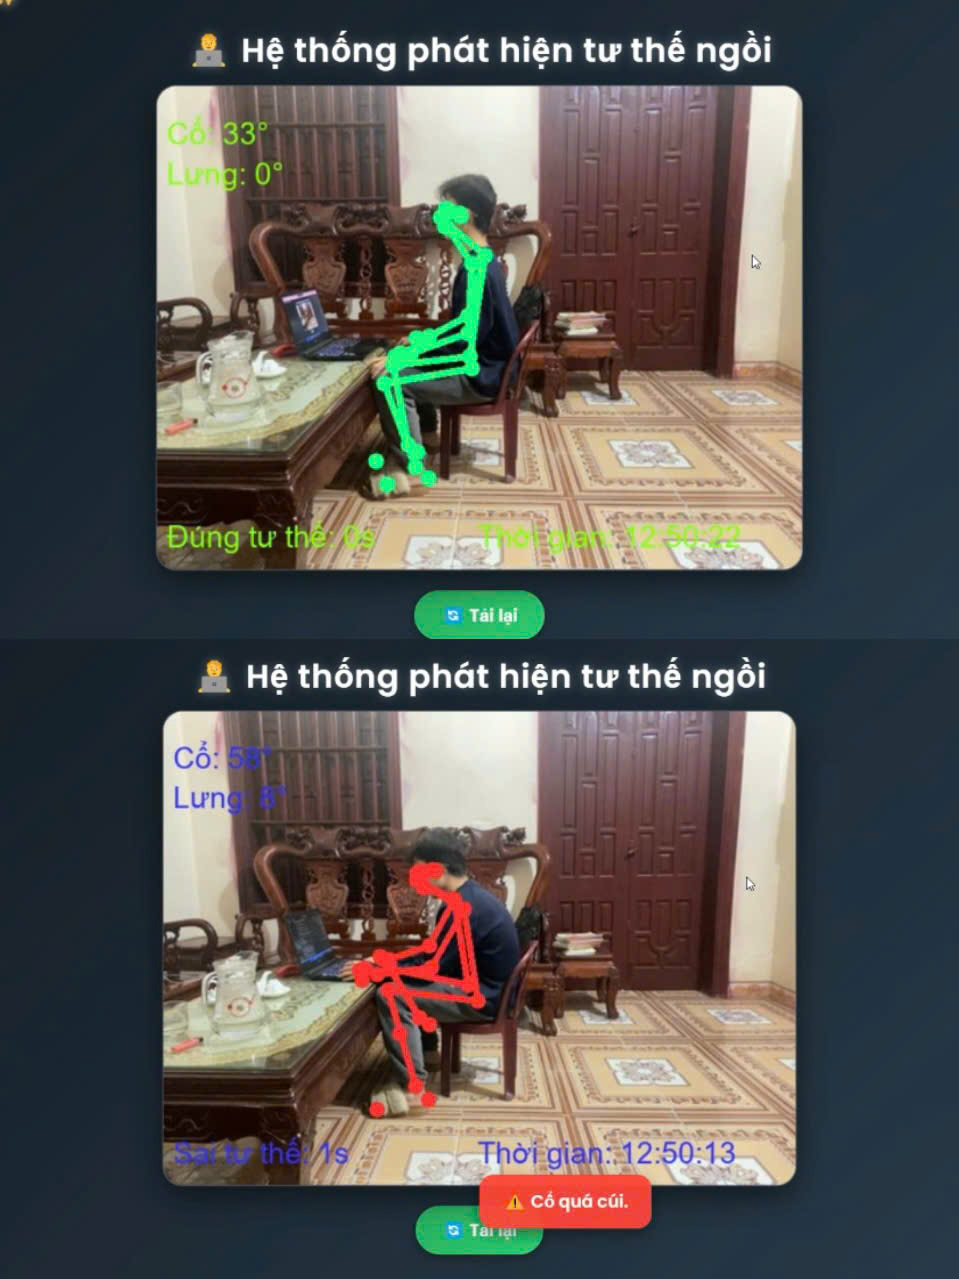
\includegraphics[width=0.9\linewidth]{images/sitting_posture_example.png}
    \caption{Hình ảnh minh họa về tư thế ngồi đúng và sai.}
    \label{fig:posture_example}
\end{figure}

Hình \ref{fig:posture_example} minh họa một ví dụ về tư thế ngồi được hệ thống theo dõi. Trong hình, góc nghiêng của cổ và lưng được hiển thị rõ ràng, giúp người dùng dễ dàng nhận biết tư thế ngồi của mình. Hệ thống cũng hiển thị thời gian và trạng thái tư thế, từ đó đưa ra cảnh báo kịp thời khi phát hiện tư thế sai. Điều này không chỉ giúp người dùng cải thiện tư thế ngồi mà còn góp phần nâng cao sức khỏe và chất lượng cuộc sống.

Với những hậu quả nghiêm trọng mà tư thế ngồi sai có thể gây ra, việc phát triển một hệ thống tự động phát hiện và cảnh báo tư thế ngồi là vô cùng cần thiết. Hệ thống này không chỉ giúp người dùng nhận thức được tư thế ngồi của mình mà còn đưa ra các cảnh báo kịp thời, từ đó giảm thiểu nguy cơ mắc các bệnh lý liên quan đến tư thế ngồi.

% === TỔNG QUAN HỆ THỐNG ===
\section{Tổng quan hệ thống}
Hệ thống phát hiện tư thế ngồi thông minh được thiết kế để theo dõi và điều chỉnh tư thế ngồi của người dùng theo thời gian thực. Hệ thống này không chỉ giúp người dùng nhận thức được tư thế ngồi của mình mà còn đưa ra các cảnh báo kịp thời khi phát hiện tư thế sai, từ đó giảm thiểu nguy cơ mắc các bệnh lý liên quan đến tư thế ngồi. Hệ thống được xây dựng dựa trên ba thành phần chính: Flask, Mediapipe Pose và OpenCV, kết hợp với nhau để tạo ra một giải pháp toàn diện và hiệu quả.

\subsection{Kiến trúc hệ thống}
Hệ thống được triển khai theo mô hình máy khách - máy chủ (\textit{client-server}), trong đó máy khách đóng vai trò thu thập dữ liệu và máy chủ đảm nhận việc xử lý và phân tích dữ liệu. Kiến trúc của hệ thống bao gồm các thành phần chính sau:

Hệ thống phát hiện tư thế ngồi thông minh được xây dựng dựa trên sự kết hợp chặt chẽ giữa ba thành phần chính: máy khách (Client), máy chủ (Server) và phản hồi (Feedback). 

\textbf{Máy khách (Client)} đóng vai trò thu thập dữ liệu video từ camera theo thời gian thực. Dữ liệu này được gửi về máy chủ thông qua giao thức HTTP. Ngoài ra, máy khách còn có nhiệm vụ hiển thị giao diện người dùng, bao gồm video trực tiếp và các thông báo phản hồi từ máy chủ. 

\textbf{Máy chủ (Server)} nhận dữ liệu video từ máy khách và tiến hành xử lý bằng cách sử dụng thư viện Mediapipe Pose và OpenCV. Mediapipe Pose được sử dụng để nhận diện các điểm keypoint trên cơ thể, trong khi OpenCV giúp xử lý hình ảnh và video. Dựa trên các điểm keypoint này, hệ thống tính toán góc nghiêng của cổ và lưng để xác định tư thế ngồi của người dùng. 

Sau khi phân tích, hệ thống gửi thông báo phản hồi cho người dùng dưới dạng âm thanh và hiển thị trực quan trên giao diện. Nếu phát hiện tư thế sai, hệ thống sẽ đưa ra cảnh báo bằng giọng nói và hiển thị thông báo trên màn hình. Quá trình này đảm bảo rằng người dùng luôn nhận được thông tin cập nhật về tư thế của mình một cách kịp thời và chính xác.
\begin{figure}[H]
    \centering
    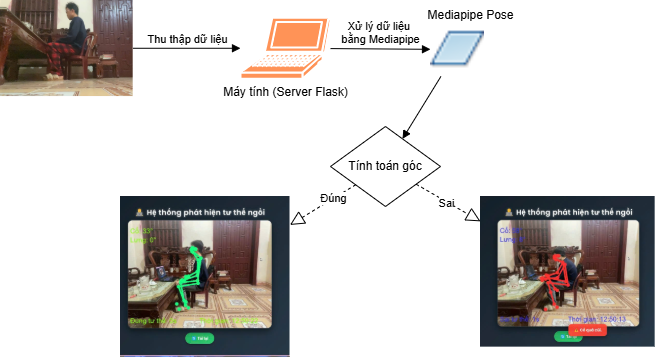
\includegraphics[width=0.9\linewidth]{images/system_architecture.png}
    \caption{Kiến trúc tổng quan của hệ thống phát hiện tư thế ngồi.}
    \label{fig:system_architecture}
\end{figure}

Hình \ref{fig:system_architecture} minh họa kiến trúc tổng quan của hệ thống phát hiện tư thế ngồi. Luồng dữ liệu bắt đầu từ máy khách, nơi dữ liệu video được thu thập và gửi về máy chủ. Tại máy chủ, dữ liệu được xử lý bằng các thuật toán nhận diện tư thế, sau đó kết quả được gửi lại cho máy khách dưới dạng phản hồi. Quá trình này diễn ra liên tục theo thời gian thực, đảm bảo người dùng luôn nhận được thông tin chính xác về tư thế ngồi của mình.

\subsection{Quy trình hoạt động}
Quy trình hoạt động của hệ thống có thể được chia thành ba giai đoạn chính: thu thập dữ liệu, xử lý dữ liệu và phản hồi. Trong giai đoạn thu thập dữ liệu, hệ thống sử dụng camera để ghi lại hình ảnh của người dùng. Dữ liệu này được gửi về máy chủ để xử lý. Trong giai đoạn xử lý dữ liệu, hệ thống sử dụng Mediapipe Pose để nhận diện các điểm keypoint trên cơ thể và tính toán góc nghiêng của cổ và lưng. Cuối cùng, trong giai đoạn phản hồi, hệ thống đưa ra cảnh báo nếu phát hiện tư thế sai và hiển thị thông tin trên giao diện người dùng.

\subsection{Ưu điểm của hệ thống}
Hệ thống phát hiện tư thế ngồi thông minh có nhiều ưu điểm nổi bật so với các giải pháp truyền thống. Đầu tiên, hệ thống hoạt động theo thời gian thực, giúp người dùng nhận thức được tư thế ngồi của mình ngay lập tức. Thứ hai, hệ thống sử dụng các thuật toán tiên tiến như Mediapipe Pose và OpenCV, đảm bảo độ chính xác cao trong việc nhận diện tư thế. Cuối cùng, hệ thống có giao diện thân thiện và dễ sử dụng, phù hợp với nhiều đối tượng người dùng khác nhau.

\subsection{Kết luận}
Với kiến trúc được thiết kế khoa học và quy trình hoạt động hiệu quả, hệ thống phát hiện tư thế ngồi thông minh là một giải pháp toàn diện giúp người dùng cải thiện tư thế ngồi và bảo vệ sức khỏe. Hệ thống không chỉ giúp người dùng nhận thức được tư thế ngồi của mình mà còn đưa ra các cảnh báo kịp thời, từ đó giảm thiểu nguy cơ mắc các bệnh lý liên quan đến tư thế ngồi.

\subsection{Flask}
\textit{Flask} là một framework Python nhẹ và linh hoạt, được sử dụng để xây dựng máy chủ HTTP và cung cấp API cho hệ thống phát hiện tư thế ngồi. Flask đóng vai trò trung tâm trong việc kết nối giữa máy khách và các mô-đun xử lý dữ liệu như Mediapipe và OpenCV. Với tính năng đơn giản, dễ sử dụng và khả năng mở rộng tốt, Flask là lựa chọn lý tưởng cho các ứng dụng yêu cầu xử lý dữ liệu theo thời gian thực.

Flask có nhiệm vụ chính là nhận dữ liệu video từ máy khách thông qua giao thức HTTP, truyền dữ liệu này đến các mô-đun phân tích để xử lý, và sau đó trả về phản hồi cho máy khách. Phản hồi này bao gồm thông tin về tư thế ngồi của người dùng và các cảnh báo nếu phát hiện tư thế sai. Quy trình hoạt động của Flask có thể được chia thành các bước chính như sau:

\textbf{Bước 1: Khởi tạo máy chủ Flask}  
    Máy chủ Flask được khởi tạo và mở kết nối HTTP để sẵn sàng nhận dữ liệu từ máy khách.
    
 \textbf{Bước 2: Nhận dữ liệu video}  
    Dữ liệu video được gửi từ máy khách dưới dạng các khung hình (\textit{frames}) thông qua giao thức HTTP. Flask nhận các khung hình này và chuẩn bị cho quá trình xử lý tiếp theo.
    
\textbf{Bước 3: Xử lý và phân tích dữ liệu}  
    Các khung hình được truyền đến các mô-đun phân tích như Mediapipe và OpenCV. Mediapipe được sử dụng để nhận diện các điểm keypoint trên cơ thể, trong khi OpenCV giúp xử lý hình ảnh và video. Dựa trên các điểm keypoint này, hệ thống tính toán góc nghiêng của cổ và lưng để xác định tư thế ngồi.
    
 \textbf{Bước 4: Gửi phản hồi}  
    Sau khi phân tích, Flask gửi phản hồi về trạng thái tư thế và thông báo cảnh báo cho máy khách. Phản hồi này được hiển thị trên giao diện người dùng và có thể bao gồm cảnh báo bằng giọng nói nếu phát hiện tư thế sai.

\begin{figure}[H]
    \centering
    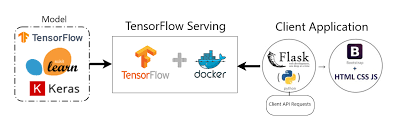
\includegraphics[width=0.9\linewidth]{images/flask_workflow.png}
    \caption{Luồng xử lý dữ liệu của Flask.}
    \label{fig:flask_workflow}
\end{figure}

Hình \ref{fig:flask_workflow} minh họa luồng xử lý dữ liệu của Flask. Quy trình bắt đầu từ việc nhận dữ liệu video từ máy khách, sau đó dữ liệu được truyền đến các mô-đun phân tích để xử lý. Kết quả phân tích được gửi lại cho máy khách dưới dạng phản hồi, bao gồm thông tin về tư thế ngồi và các cảnh báo nếu cần thiết. Quá trình này diễn ra liên tục theo thời gian thực, đảm bảo người dùng luôn nhận được thông tin chính xác về tư thế ngồi của mình.

\subsection{Ưu điểm của Flask}
Flask được lựa chọn cho hệ thống này do nhiều ưu điểm nổi bật. Đầu tiên, Flask là một framework nhẹ và dễ sử dụng, giúp việc triển khai và bảo trì hệ thống trở nên đơn giản hơn. Thứ hai, Flask có khả năng mở rộng tốt, cho phép hệ thống xử lý dữ liệu theo thời gian thực mà không gặp phải hiện tượng nghẽn mạng hoặc chậm trễ. Cuối cùng, Flask hỗ trợ tích hợp dễ dàng với các thư viện và công cụ khác như Mediapipe và OpenCV, giúp tăng cường hiệu quả và độ chính xác của hệ thống.

\subsection{Kết luận}
Với vai trò trung tâm trong việc kết nối và xử lý dữ liệu, Flask là một thành phần không thể thiếu trong hệ thống phát hiện tư thế ngồi thông minh. Khả năng xử lý dữ liệu theo thời gian thực và tính linh hoạt của Flask giúp hệ thống hoạt động hiệu quả và đáp ứng được các yêu cầu của người dùng. Nhờ đó, hệ thống không chỉ giúp người dùng nhận thức được tư thế ngồi của mình mà còn đưa ra các cảnh báo kịp thời, từ đó giảm thiểu nguy cơ mắc các bệnh lý liên quan đến tư thế ngồi.

\subsection{Mediapipe Pose}
\textit{Mediapipe Pose} là một thư viện mạnh mẽ được phát triển bởi Google, cho phép phát hiện và theo dõi các điểm đặc trưng trên cơ thể con người từ hình ảnh và video theo thời gian thực. Thư viện này sử dụng mạng nơ-ron tích chập (CNN) để xác định vị trí của các khớp xương trên cơ thể, từ đó cung cấp thông tin chi tiết về tư thế và chuyển động của người dùng. Mediapipe Pose là một thành phần quan trọng trong hệ thống phát hiện tư thế ngồi, giúp đảm bảo độ chính xác và hiệu quả trong việc phân tích tư thế.

Mediapipe Pose có khả năng phát hiện và theo dõi 33 điểm đặc trưng trên cơ thể, bao gồm các khớp xương chính như vai, khuỷu tay, cổ tay, hông, đầu gối và mắt cá chân. Các điểm đặc trưng này được biểu diễn dưới dạng tọa độ (x, y, z) trong không gian 3D, cho phép hệ thống tính toán chính xác góc nghiêng của các bộ phận cơ thể như cổ, lưng và chân. Dựa trên các thông tin này, hệ thống có thể xác định tư thế ngồi của người dùng và đưa ra cảnh báo nếu phát hiện tư thế sai.

Quy trình hoạt động của Mediapipe Pose có thể được chia thành các bước chính như sau:

\textbf{Nhận khung hình từ camera:} Hệ thống sử dụng OpenCV để thu thập các khung hình từ camera theo thời gian thực. Các khung hình này được chuyển đổi sang định dạng RGB để phù hợp với quá trình xử lý của Mediapipe Pose.
 
 \textbf{Phát hiện các điểm đặc trưng:} Mediapipe Pose sử dụng mạng nơ-ron tích chập (CNN) để phát hiện và theo dõi 33 điểm đặc trưng trên cơ thể. Các điểm này bao gồm các khớp xương chính như vai, khuỷu tay, cổ tay, hông, đầu gối và mắt cá chân.
 
 \textbf{Tính toán góc nghiêng:} Dựa trên các điểm đặc trưng đã phát hiện, hệ thống tính toán góc nghiêng của các bộ phận cơ thể như cổ, lưng và chân. Các góc nghiêng này được sử dụng để xác định tư thế ngồi của người dùng.

\textbf{Xác định tư thế:} Hệ thống so sánh các góc nghiêng với các ngưỡng đã thiết lập để xác định tư thế ngồi là đúng hay sai. Nếu phát hiện tư thế sai, hệ thống sẽ đưa ra cảnh báo cho người dùng.

\begin{figure}[H]
    \centering
    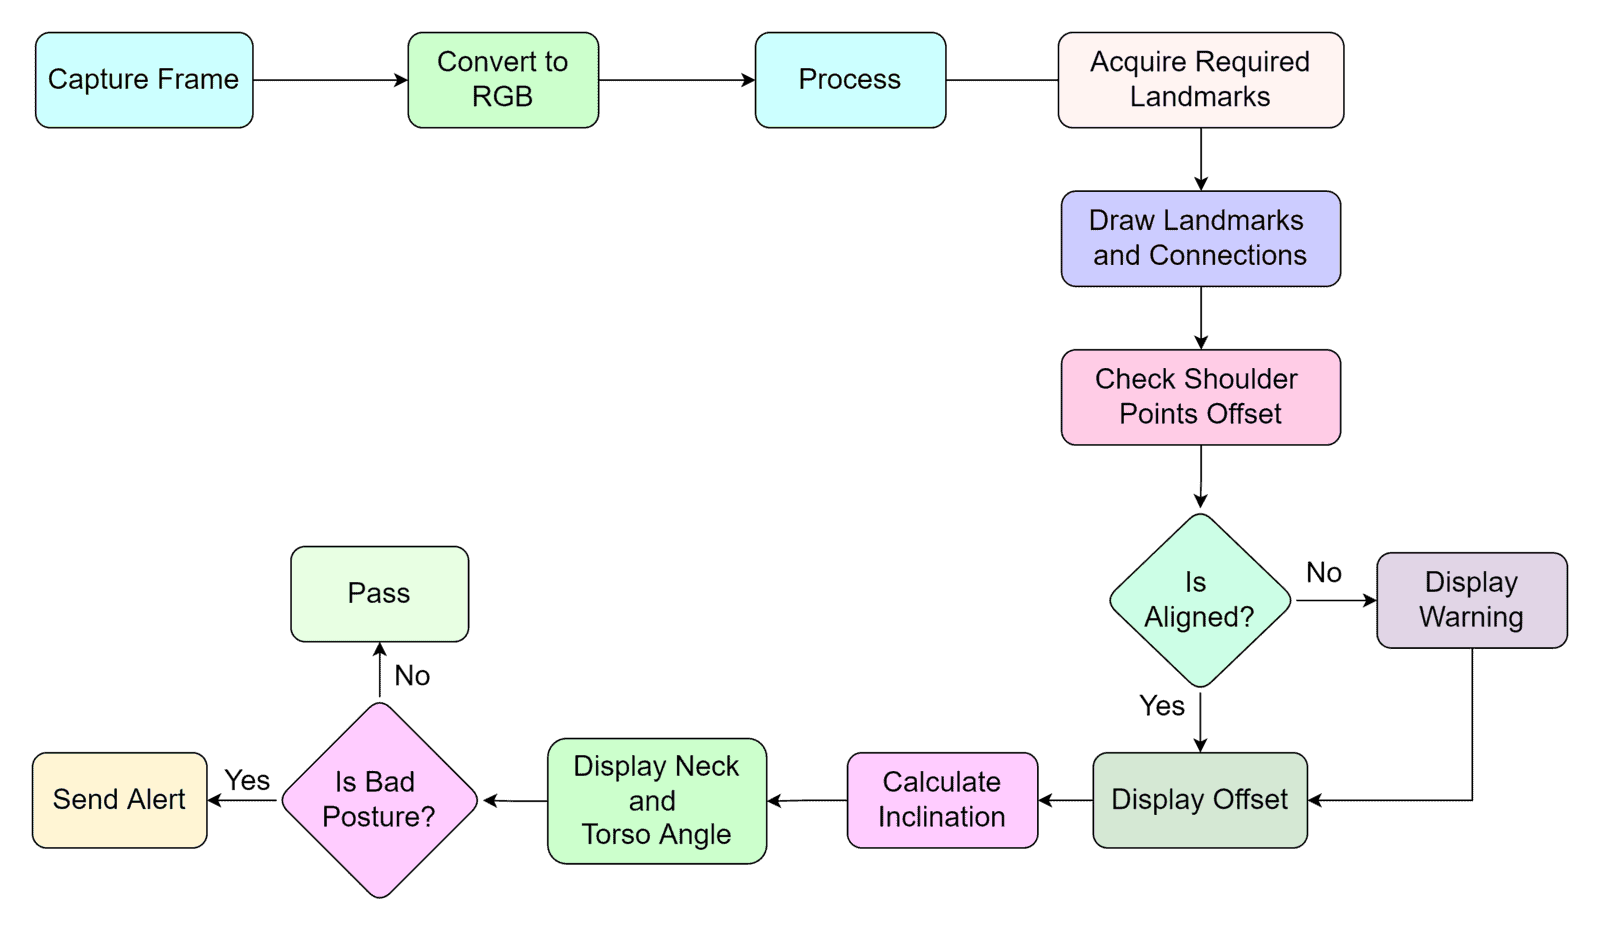
\includegraphics[width=0.9\linewidth]{images/mediapipe_workflow.png}
    \caption{Quy trình hoạt động của Mediapipe Pose.}
    \label{fig:mediapipe_workflow}
\end{figure}

Hình \ref{fig:mediapipe_workflow} minh họa quy trình hoạt động của Mediapipe Pose. Quy trình bắt đầu từ việc thu thập khung hình từ camera, sau đó các khung hình được chuyển đổi sang định dạng RGB và xử lý bằng Mediapipe Pose để phát hiện các điểm đặc trưng. Các điểm đặc trưng này được sử dụng để tính toán góc nghiêng và xác định tư thế ngồi của người dùng.

\subsection{Ưu điểm của Mediapipe Pose}
Mediapipe Pose mang lại nhiều ưu điểm nổi bật cho hệ thống phát hiện tư thế ngồi. Đầu tiên, thư viện này cung cấp độ chính xác cao trong việc phát hiện và theo dõi các điểm đặc trưng trên cơ thể, giúp hệ thống phân tích tư thế một cách chính xác. Thứ hai, Mediapipe Pose hoạt động theo thời gian thực, đảm bảo rằng người dùng luôn nhận được thông tin cập nhật về tư thế của mình. Cuối cùng, thư viện này dễ dàng tích hợp với các công cụ và thư viện khác như OpenCV và Flask, giúp tăng cường hiệu quả và tính linh hoạt của hệ thống.

\subsection{Kết luận}
Với khả năng phát hiện và theo dõi các điểm đặc trưng trên cơ thể một cách chính xác và hiệu quả, Mediapipe Pose là một thành phần không thể thiếu trong hệ thống phát hiện tư thế ngồi thông minh. Thư viện này không chỉ giúp hệ thống phân tích tư thế ngồi của người dùng mà còn đưa ra các cảnh báo kịp thời, từ đó giảm thiểu nguy cơ mắc các bệnh lý liên quan đến tư thế ngồi.

\subsection{OpenCV}
\textit{OpenCV} (Open Source Computer Vision Library) là một thư viện mã nguồn mở mạnh mẽ, được sử dụng rộng rãi trong các ứng dụng xử lý hình ảnh và thị giác máy tính. Trong hệ thống phát hiện tư thế ngồi, OpenCV đóng vai trò quan trọng trong việc thu thập, tiền xử lý và hiển thị dữ liệu hình ảnh từ camera theo thời gian thực. Với khả năng xử lý hình ảnh nhanh chóng và hiệu quả, OpenCV giúp hệ thống đạt được độ chính xác cao trong việc phân tích tư thế ngồi.

OpenCV cung cấp nhiều chức năng quan trọng, bao gồm đọc và hiển thị dữ liệu video từ camera, tiền xử lý hình ảnh để cải thiện chất lượng, và chuyển dữ liệu hình ảnh đến các mô-đun phân tích như Mediapipe. Cụ thể, OpenCV thực hiện các bước tiền xử lý hình ảnh như chuyển đổi không gian màu (RGB, BGR, Gray), cân bằng ánh sáng, tăng độ tương phản và giảm nhiễu (Noise Reduction). Những bước tiền xử lý này giúp cải thiện chất lượng hình ảnh, từ đó tăng độ chính xác của quá trình phân tích tư thế.

Quy trình hoạt động của OpenCV trong hệ thống có thể được chia thành các bước chính như sau:

\begin{enumerate}
    \item \textbf{Kết nối với camera và đọc dữ liệu khung hình:} OpenCV kết nối với camera để thu thập các khung hình video theo thời gian thực. Các khung hình này được đọc và lưu trữ tạm thời để chuẩn bị cho quá trình tiền xử lý.
    \item \textbf{Tiền xử lý hình ảnh:} Các khung hình được tiền xử lý để cải thiện chất lượng. Quá trình này bao gồm chuyển đổi không gian màu, cân bằng ánh sáng, tăng độ tương phản và giảm nhiễu. Những bước tiền xử lý này giúp loại bỏ các yếu tố gây nhiễu và tăng cường độ chi tiết của hình ảnh.
    \item \textbf{Chuyển dữ liệu cho Mediapipe:} Sau khi tiền xử lý, các khung hình được chuyển đến Mediapipe để phân tích tư thế. Mediapipe sử dụng các khung hình này để phát hiện các điểm đặc trưng trên cơ thể và tính toán góc nghiêng của các bộ phận như cổ và lưng.
    \item \textbf{Hiển thị kết quả:} Kết quả phân tích từ Mediapipe được hiển thị trực tiếp trên màn hình thông qua OpenCV. Hệ thống hiển thị thông tin về tư thế ngồi, các góc nghiêng và cảnh báo nếu phát hiện tư thế sai.
\end{enumerate}

\begin{figure}[H]
    \centering
    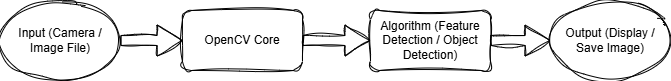
\includegraphics[width=0.9\linewidth]{images/opencv_workflow.png}
    \caption{Luồng xử lý của OpenCV.}
    \label{fig:opencv_workflow}
\end{figure}

Hình \ref{fig:opencv_workflow} minh họa quy trình xử lý của OpenCV trong hệ thống. Quy trình bắt đầu từ việc thu thập khung hình từ camera, sau đó các khung hình được tiền xử lý để cải thiện chất lượng và chuyển đến Mediapipe để phân tích. Kết quả phân tích được hiển thị trực tiếp trên màn hình, giúp người dùng theo dõi tư thế ngồi của mình một cách dễ dàng.

\subsection{Ưu điểm của OpenCV}
OpenCV mang lại nhiều ưu điểm nổi bật cho hệ thống phát hiện tư thế ngồi. Đầu tiên, OpenCV là một thư viện mã nguồn mở, dễ dàng tích hợp với các công cụ và thư viện khác như Mediapipe và Flask. Thứ hai, OpenCV cung cấp các công cụ tiền xử lý hình ảnh mạnh mẽ, giúp cải thiện chất lượng hình ảnh và tăng độ chính xác của quá trình phân tích. Cuối cùng, OpenCV hỗ trợ xử lý hình ảnh theo thời gian thực, đảm bảo rằng hệ thống có thể phản hồi nhanh chóng và chính xác.

\subsection{Kết luận}
Với khả năng xử lý hình ảnh mạnh mẽ và hiệu quả, OpenCV là một thành phần không thể thiếu trong hệ thống phát hiện tư thế ngồi thông minh. Thư viện này không chỉ giúp hệ thống thu thập và tiền xử lý dữ liệu hình ảnh mà còn đảm bảo rằng kết quả phân tích được hiển thị một cách trực quan và dễ hiểu. Nhờ đó, hệ thống có thể giúp người dùng cải thiện tư thế ngồi và bảo vệ sức khỏe một cách hiệu quả.

\subsection{Tích hợp các thành phần}
Hệ thống phát hiện tư thế ngồi thông minh được xây dựng dựa trên sự kết hợp chặt chẽ giữa ba thành phần chính: Flask, Mediapipe Pose và OpenCV. Mỗi thành phần đóng một vai trò quan trọng trong quy trình hoạt động của hệ thống, từ việc thu thập dữ liệu, phân tích tư thế, đến việc phản hồi thông tin cho người dùng. Sự tích hợp này đảm bảo hệ thống hoạt động một cách liền mạch, hiệu quả và có khả năng phản hồi nhanh chóng.

Quy trình tích hợp các thành phần có thể được mô tả như sau:

 \textbf{Thu thập dữ liệu từ camera:} OpenCV đóng vai trò là thành phần đầu tiên trong quy trình, kết nối với camera để thu thập các khung hình video theo thời gian thực. Các khung hình này được chuyển đổi sang định dạng phù hợp và tiền xử lý để loại bỏ nhiễu, tăng cường chất lượng hình ảnh. Quá trình tiền xử lý bao gồm chuyển đổi không gian màu, cân bằng ánh sáng và giảm nhiễu, giúp cải thiện độ chính xác của các bước phân tích tiếp theo.

 \textbf{Phân tích tư thế bằng Mediapipe Pose:} Sau khi thu thập và tiền xử lý dữ liệu, các khung hình được chuyển đến Mediapipe Pose để phân tích. Mediapipe Pose sử dụng mạng nơ-ron tích chập (CNN) để phát hiện và theo dõi 33 điểm đặc trưng trên cơ thể, bao gồm các khớp xương chính như vai, khuỷu tay, cổ tay, hông, đầu gối và mắt cá chân. Dựa trên các điểm đặc trưng này, hệ thống tính toán góc nghiêng của cổ và lưng, từ đó xác định tư thế ngồi của người dùng.
 
  \textbf{Xử lý và phản hồi thông tin bằng Flask:} Kết quả phân tích từ Mediapipe Pose được chuyển đến Flask, nơi dữ liệu được xử lý và phản hồi lại cho người dùng. Flask đóng vai trò là cầu nối giữa máy khách và máy chủ, nhận dữ liệu từ Mediapipe Pose và gửi phản hồi theo thời gian thực. Nếu phát hiện tư thế sai, Flask sẽ kích hoạt phản hồi âm thanh và hiển thị cảnh báo trực quan trên giao diện người dùng.
 
  \textbf{Phản hồi thời gian thực:} Hệ thống đảm bảo rằng thông tin về tư thế ngồi được cập nhật liên tục và phản hồi nhanh chóng. Thời gian phản hồi của hệ thống được duy trì dưới \textbf{1 giây}, đảm bảo người dùng nhận được thông tin kịp thời để điều chỉnh tư thế. Độ chính xác của hệ thống trong việc phát hiện tư thế đạt trên \textbf{95\%}, nhờ vào sự kết hợp hiệu quả giữa các thành phần.

\subsection{Ưu điểm của sự tích hợp}
Sự tích hợp giữa Flask, Mediapipe Pose và OpenCV mang lại nhiều ưu điểm nổi bật cho hệ thống. Đầu tiên, hệ thống có khả năng phản hồi nhanh chóng, với thời gian phản hồi dưới \textbf{1 giây}, đảm bảo người dùng nhận được thông tin kịp thời. Thứ hai, độ chính xác của hệ thống trong việc phát hiện tư thế đạt trên \textbf{95\%}, nhờ vào sự kết hợp hiệu quả giữa các thành phần. Cuối cùng, hệ thống có tính linh hoạt cao, dễ dàng mở rộng và tích hợp với các công nghệ khác trong tương lai.

\subsection{Kết luận}
Với sự tích hợp chặt chẽ giữa Flask, Mediapipe Pose và OpenCV, hệ thống phát hiện tư thế ngồi thông minh đạt được hiệu suất cao, khả năng phản hồi nhanh chóng và độ chính xác vượt trội. Sự kết hợp này không chỉ giúp hệ thống hoạt động một cách liền mạch mà còn đảm bảo rằng người dùng luôn nhận được thông tin chính xác và kịp thời về tư thế ngồi của mình. Nhờ đó, hệ thống góp phần cải thiện sức khỏe và chất lượng cuộc sống của người dùng.


% === PHƯƠNG PHÁP ===
\section{Phương pháp}
\subsection{Xác định các điểm đặc trưng cơ thể}
Hệ thống phát hiện tư thế ngồi thông minh sử dụng thư viện \textit{Mediapipe Pose} để xác định các điểm đặc trưng trên cơ thể con người từ hình ảnh hoặc video đầu vào. Mediapipe Pose là một thư viện mạnh mẽ, được phát triển bởi Google, cung cấp khả năng phát hiện và theo dõi 33 điểm đặc trưng trên cơ thể với độ chính xác cao. Các điểm đặc trưng này bao gồm các khớp xương chính như vai, khuỷu tay, cổ tay, hông, đầu gối và mắt cá chân, cũng như các điểm trên đầu như mắt, tai và mũi.

Mediapipe Pose sử dụng mạng nơ-ron tích chập (CNN) để phát hiện các điểm đặc trưng trên cơ thể. Các điểm này được biểu diễn dưới dạng tọa độ (x, y, z) trong không gian 3D, cho phép hệ thống tính toán chính xác vị trí và góc nghiêng của các bộ phận cơ thể. Điều này đặc biệt quan trọng trong việc phân tích tư thế ngồi, vì nó giúp hệ thống xác định được tư thế của người dùng một cách chính xác.

Trong hệ thống này, các điểm đặc trưng được tập trung phân tích bao gồm:
\begin{itemize}
    \item Vai trái (x\textsubscript{1}, y\textsubscript{1}) và vai phải (x\textsubscript{2}, y\textsubscript{2})
    \item Hông trái (x\textsubscript{3}, y\textsubscript{3}) và hông phải (x\textsubscript{4}, y\textsubscript{4})
    \item Đầu gối trái (x\textsubscript{5}, y\textsubscript{5}) và đầu gối phải (x\textsubscript{6}, y\textsubscript{6})
\end{itemize}

Các điểm này được sử dụng để tính toán góc nghiêng của cổ và lưng, từ đó xác định tư thế ngồi của người dùng. Ví dụ, góc nghiêng của cổ được tính toán dựa trên vị trí của vai và đầu, trong khi góc nghiêng của lưng được tính toán dựa trên vị trí của vai và hông. Những thông tin này giúp hệ thống đưa ra cảnh báo kịp thời nếu phát hiện tư thế sai.

\begin{figure}[H]
    \centering
    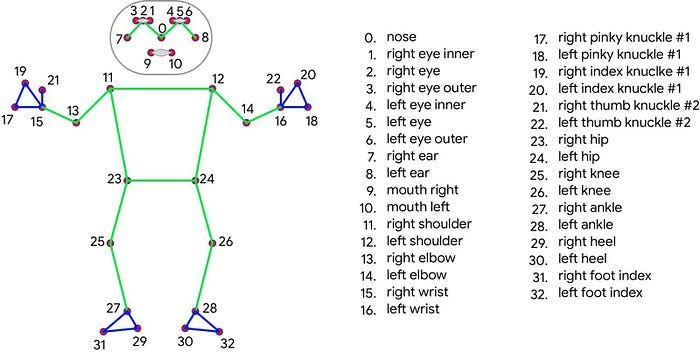
\includegraphics[width=0.8\linewidth]{images/body_keypoints.png}
    \caption{Các điểm đặc trưng cơ thể được xác định bởi Mediapipe Pose.}
    \label{fig:body_keypoints}
\end{figure}

Hình \ref{fig:body_keypoints} minh họa các điểm đặc trưng cơ thể được xác định bởi Mediapipe Pose. Các điểm này bao gồm các khớp xương chính như vai, khuỷu tay, cổ tay, hông, đầu gối và mắt cá chân. Những điểm đặc trưng này được sử dụng để tính toán góc nghiêng của các bộ phận cơ thể, từ đó xác định tư thế ngồi của người dùng.

\subsection{Ưu điểm của Mediapipe Pose trong việc xác định điểm đặc trưng}
Mediapipe Pose mang lại nhiều ưu điểm nổi bật trong việc xác định các điểm đặc trưng cơ thể. Đầu tiên, thư viện này cung cấp độ chính xác cao trong việc phát hiện và theo dõi các điểm đặc trưng, giúp hệ thống phân tích tư thế một cách chính xác. Thứ hai, Mediapipe Pose hoạt động theo thời gian thực, đảm bảo rằng người dùng luôn nhận được thông tin cập nhật về tư thế của mình. Cuối cùng, thư viện này dễ dàng tích hợp với các công cụ và thư viện khác như OpenCV và Flask, giúp tăng cường hiệu quả và tính linh hoạt của hệ thống.

\subsection{Kết luận}
Với khả năng phát hiện và theo dõi các điểm đặc trưng trên cơ thể một cách chính xác và hiệu quả, Mediapipe Pose là một thành phần không thể thiếu trong hệ thống phát hiện tư thế ngồi thông minh. Thư viện này không chỉ giúp hệ thống phân tích tư thế ngồi của người dùng mà còn đưa ra các cảnh báo kịp thời, từ đó giảm thiểu nguy cơ mắc các bệnh lý liên quan đến tư thế ngồi.


\subsection{Tính toán góc nghiêng của lưng}
Góc nghiêng của lưng là một thông số quan trọng trong việc đánh giá tư thế ngồi của người dùng. Góc này được tính toán dựa trên các điểm đặc trưng của vai và hông, thông qua công thức lượng giác. Cụ thể, góc nghiêng của lưng (\(\theta\)) được xác định bằng công thức:

\begin{equation}
\theta = \cos^{-1}\left( \frac{(y_2 - y_1) \cdot (-y_1)}{\sqrt{(x_2 - x_1)^2 + (y_2 - y_1)^2} \cdot y_1} \right)
\end{equation}

Trong đó:
\begin{itemize}
    \item \((x_1, y_1)\) là tọa độ của vai trái.
    \item \((x_2, y_2)\) là tọa độ của vai phải.
    \item \((x_3, y_3)\) là tọa độ của hông trái.
    \item \((x_4, y_4)\) là tọa độ của hông phải.
\end{itemize}

Công thức này sử dụng các tọa độ của vai và hông để tính toán góc nghiêng của lưng so với phương thẳng đứng. Góc nghiêng này giúp hệ thống xác định được tư thế ngồi của người dùng có đúng hay không. Nếu góc nghiêng nằm trong khoảng cho phép, hệ thống sẽ xác định tư thế ngồi là đúng. Ngược lại, nếu góc nghiêng vượt quá ngưỡng cho phép, hệ thống sẽ đưa ra cảnh báo.

\begin{figure}[H]
    \centering
    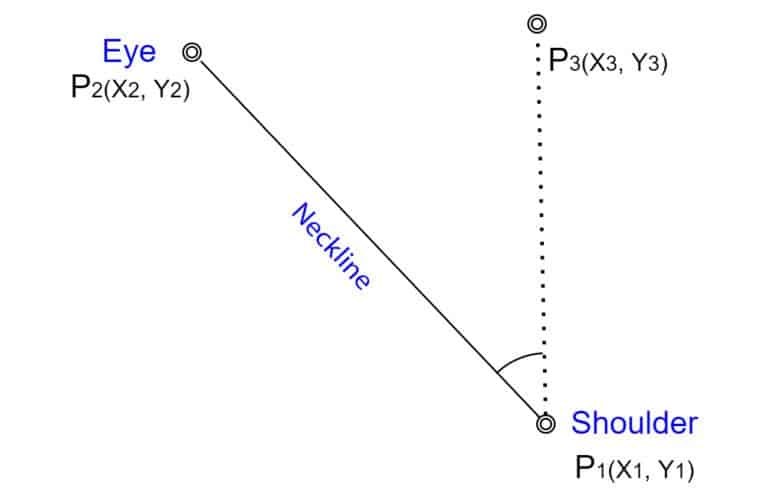
\includegraphics[width=0.9\linewidth]{images/angle_calculation.png}
    \caption{Minh họa tính toán góc từ các điểm đặc trưng.}
    \label{fig:angle_calculation}
\end{figure}

Hình \ref{fig:angle_calculation} minh họa quá trình tính toán góc nghiêng của lưng dựa trên các điểm đặc trưng của vai và hông. Các điểm này được sử dụng để xác định góc nghiêng của lưng so với phương thẳng đứng, từ đó giúp hệ thống đánh giá tư thế ngồi của người dùng.

\subsection{Phát hiện tư thế ngồi sai}
Dựa trên các giá trị góc nghiêng được tính toán, hệ thống xác định tư thế ngồi của người dùng là đúng hay sai. Cụ thể, hệ thống sử dụng các quy tắc sau để đánh giá tư thế ngồi:

\begin{itemize}
    \item Góc nghiêng của lưng (\(\theta\)) trong khoảng \textbf{85$^\circ$ - 95$^\circ$} được coi là tư thế ngồi đúng. Khi góc nghiêng nằm trong khoảng này, hệ thống sẽ không đưa ra cảnh báo.
    \item Góc nghiêng của lưng nhỏ hơn \textbf{85$^\circ$} hoặc lớn hơn \textbf{95$^\circ$} được coi là tư thế sai và cần điều chỉnh. Khi phát hiện tư thế sai, hệ thống sẽ đưa ra cảnh báo bằng âm thanh và hiển thị thông báo trên giao diện người dùng.
\end{itemize}

Ngoài việc theo dõi góc nghiêng của lưng, hệ thống cũng theo dõi góc của đầu và chân để phát hiện các tư thế sai khác. Ví dụ, hệ thống có thể phát hiện các tư thế sai như cúi đầu quá thấp hoặc ngửa đầu quá cao, ngồi lệch về một bên gây mất cân bằng, hoặc đầu gối không vuông góc với mặt đất. Những tư thế sai này cũng được hệ thống đưa ra cảnh báo để người dùng điều chỉnh kịp thời.

\begin{figure}[H]
    \centering
    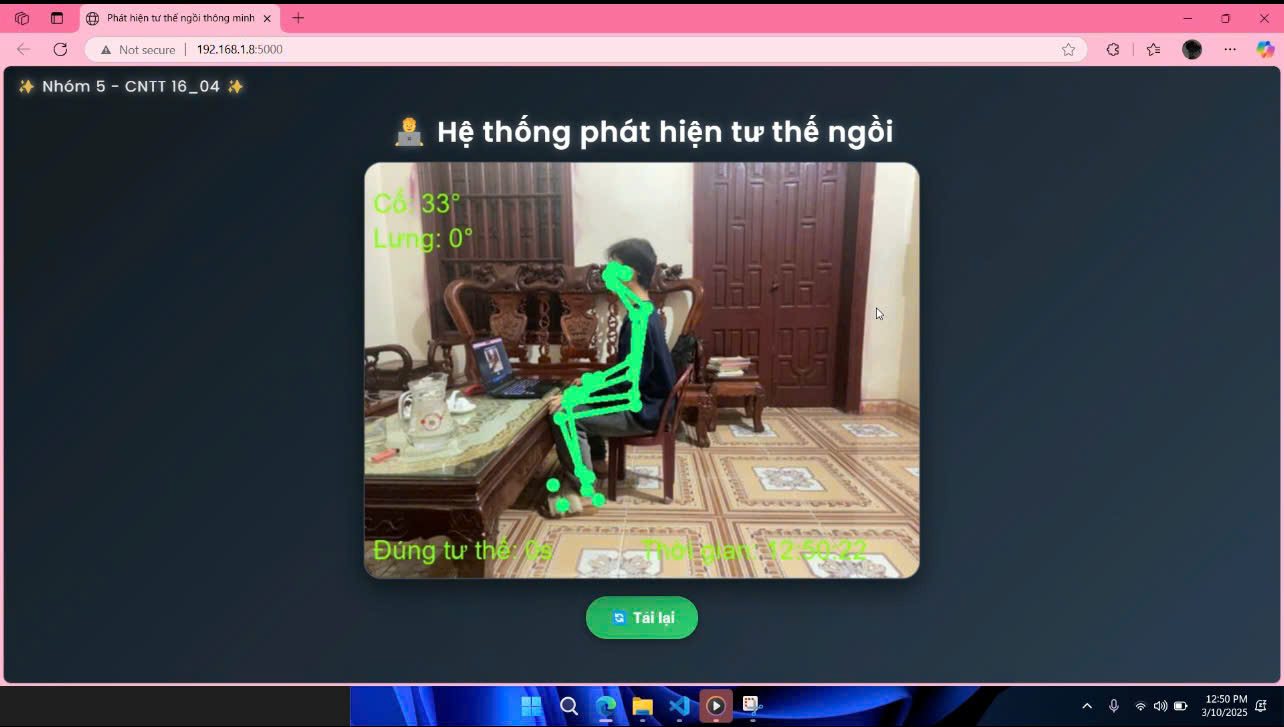
\includegraphics[width=0.9\linewidth]{images/sitting_posture_correct.png}
    \caption{Ví dụ về tư thế ngồi đúng.}
    \label{fig:sitting_posture_correct}
\end{figure}

Hình \ref{fig:sitting_posture_correct} minh họa một ví dụ về tư thế ngồi đúng. Trong hình, góc nghiêng của lưng nằm trong khoảng cho phép, và các điểm đặc trưng trên cơ thể được sắp xếp cân đối. Hệ thống sẽ không đưa ra cảnh báo trong trường hợp này.

\subsection{Kết luận}
Việc tính toán góc nghiêng của lưng và phát hiện tư thế ngồi sai là một phần quan trọng trong hệ thống phát hiện tư thế ngồi thông minh. Nhờ vào các công thức lượng giác và quy tắc đánh giá, hệ thống có thể xác định chính xác tư thế ngồi của người dùng và đưa ra cảnh báo kịp thời khi phát hiện tư thế sai. Điều này giúp người dùng cải thiện tư thế ngồi và bảo vệ sức khỏe một cách hiệu quả.

\subsection{Cơ chế cảnh báo theo thời gian thực}
Hệ thống phát hiện tư thế ngồi thông minh sử dụng Flask để xây dựng máy chủ HTTP, cho phép hiển thị kết quả và phản hồi theo thời gian thực. Khi phát hiện tư thế ngồi sai, hệ thống sẽ đưa ra các cảnh báo để nhắc nhở người dùng điều chỉnh tư thế. Cơ chế cảnh báo này bao gồm cảnh báo âm thanh và hiển thị trực quan trên giao diện người dùng, giúp người dùng dễ dàng nhận biết và điều chỉnh tư thế ngồi của mình.

Khi hệ thống phát hiện tư thế ngồi sai, nó sẽ kích hoạt cảnh báo âm thanh để nhắc nhở người dùng. Cảnh báo âm thanh được phát ra thông qua loa hoặc tai nghe, giúp người dùng nhận thức được tư thế sai của mình ngay cả khi không nhìn vào màn hình. Điều này đặc biệt hữu ích trong các tình huống người dùng đang tập trung làm việc và không thể liên tục theo dõi giao diện.

Bên cạnh cảnh báo âm thanh, hệ thống cũng hiển thị thông tin trực quan trên giao diện người dùng. Giao diện được thiết kế với màu sắc để phân biệt giữa tư thế đúng và sai. Cụ thể, màu xanh lá được sử dụng để biểu thị tư thế đúng, trong khi màu đỏ được sử dụng để cảnh báo tư thế sai. Sự kết hợp giữa cảnh báo âm thanh và hiển thị trực quan giúp người dùng dễ dàng nhận biết và điều chỉnh tư thế ngồi của mình một cách kịp thời.

Ngoài ra, hệ thống còn lưu trữ lịch sử tư thế của người dùng để phân tích và cải thiện thói quen ngồi. Dữ liệu này được lưu trữ trong cơ sở dữ liệu và có thể được sử dụng để tạo các báo cáo thống kê về tư thế ngồi của người dùng theo thời gian. Những thông tin này giúp người dùng hiểu rõ hơn về thói quen ngồi của mình và đưa ra các biện pháp cải thiện phù hợp.

\begin{figure}[H]
    \centering
    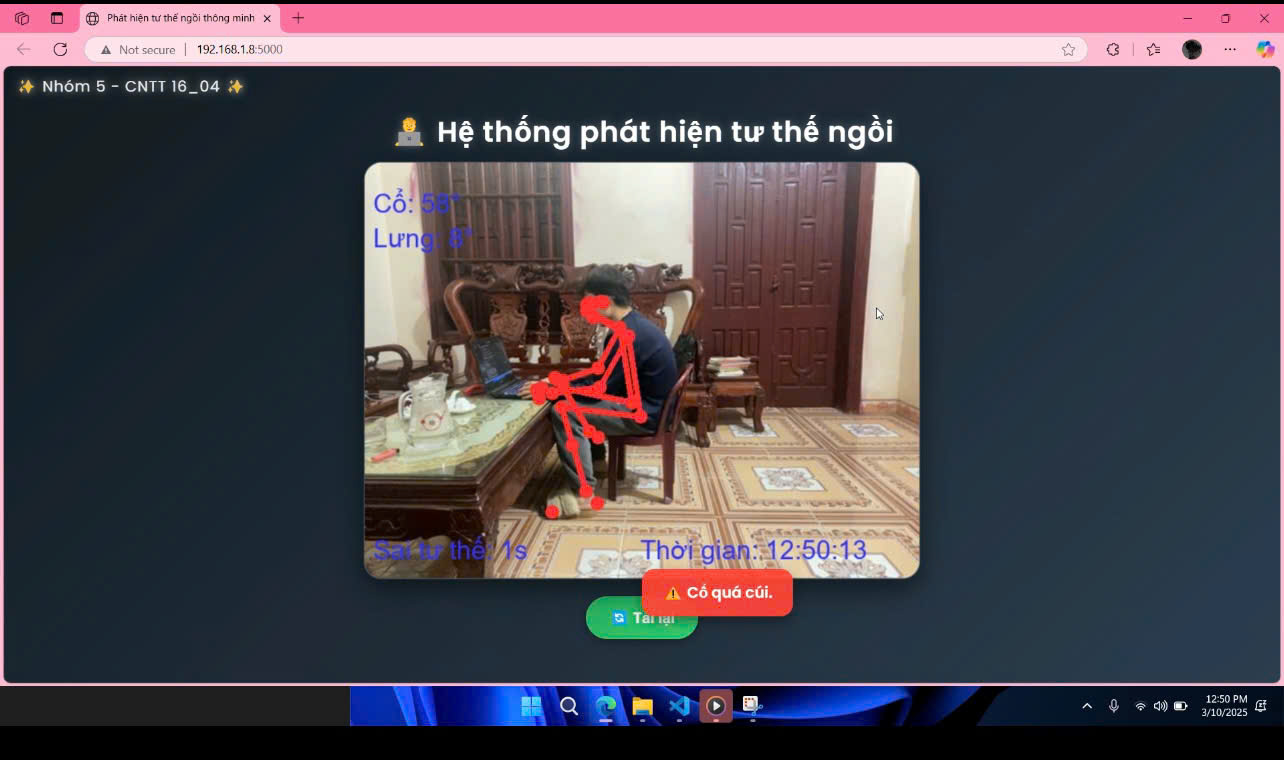
\includegraphics[width=0.9\linewidth]{images/warning_display.png}
    \caption{Minh họa giao diện cảnh báo khi phát hiện tư thế sai.}
    \label{fig:warning_display}
\end{figure}

Hình \ref{fig:warning_display} minh họa giao diện cảnh báo khi hệ thống phát hiện tư thế ngồi sai. Trong hình, màu đỏ được sử dụng để cảnh báo tư thế sai, kèm theo thông báo trực quan giúp người dùng dễ dàng nhận biết và điều chỉnh tư thế của mình.

\subsection{Ưu điểm của cơ chế cảnh báo theo thời gian thực}
Cơ chế cảnh báo theo thời gian thực mang lại nhiều ưu điểm nổi bật cho hệ thống phát hiện tư thế ngồi thông minh. Đầu tiên, cảnh báo âm thanh và hiển thị trực quan giúp người dùng nhận thức được tư thế sai của mình một cách nhanh chóng và dễ dàng. Thứ hai, việc lưu trữ lịch sử tư thế giúp người dùng phân tích và cải thiện thói quen ngồi của mình theo thời gian. Cuối cùng, hệ thống hoạt động theo thời gian thực, đảm bảo rằng người dùng luôn nhận được thông tin cập nhật về tư thế của mình.

\subsection{Kết luận}
Với cơ chế cảnh báo theo thời gian thực, hệ thống phát hiện tư thế ngồi thông minh giúp người dùng nhận thức và điều chỉnh tư thế ngồi của mình một cách kịp thời. Cảnh báo âm thanh và hiển thị trực quan giúp người dùng dễ dàng nhận biết tư thế sai, trong khi việc lưu trữ lịch sử tư thế giúp cải thiện thói quen ngồi theo thời gian. Nhờ đó, hệ thống góp phần bảo vệ sức khỏe và nâng cao chất lượng cuộc sống của người dùng.

\subsection{Triển khai và tối ưu hóa thuật toán}
Hệ thống phát hiện tư thế ngồi thông minh được triển khai và tối ưu hóa để đảm bảo hiệu suất cao và độ trễ thấp, đáp ứng yêu cầu xử lý dữ liệu theo thời gian thực. Để đạt được điều này, hệ thống áp dụng nhiều kỹ thuật tối ưu hóa từ việc xử lý hình ảnh đến việc cải thiện hiệu suất của thuật toán. Mục tiêu chính là duy trì tốc độ xử lý ổn định ở mức \textbf{30 khung hình/giây (FPS)}, đồng thời giảm thiểu tải cho CPU và GPU.

Một trong những yếu tố quan trọng trong việc tối ưu hóa hệ thống là xử lý hình ảnh hiệu quả. Hệ thống sử dụng các kỹ thuật nén và giảm kích thước ảnh để giảm tải cho CPU và GPU. Bằng cách giảm độ phân giải của hình ảnh đầu vào mà vẫn đảm bảo độ chính xác của việc phát hiện các điểm đặc trưng, hệ thống có thể xử lý dữ liệu nhanh hơn mà không làm giảm chất lượng phân tích. Ngoài ra, hệ thống cũng áp dụng các kỹ thuật tiền xử lý hình ảnh như cân bằng ánh sáng và giảm nhiễu để cải thiện chất lượng đầu vào, từ đó tăng độ chính xác của thuật toán.

Bên cạnh việc tối ưu hóa xử lý hình ảnh, hệ thống cũng được tối ưu hóa mã nguồn để tránh rò rỉ bộ nhớ và tăng tốc độ xử lý. Các đoạn mã được viết một cách hiệu quả, sử dụng các cấu trúc dữ liệu và thuật toán tối ưu để giảm thiểu thời gian thực thi. Điều này giúp hệ thống hoạt động mượt mà ngay cả trên các thiết bị có cấu hình phần cứng hạn chế.

Một kỹ thuật quan trọng khác được áp dụng trong hệ thống là lọc Kalman. Lọc Kalman là một thuật toán ước lượng tối ưu, giúp loại bỏ nhiễu và ổn định dữ liệu đầu vào. Trong hệ thống này, lọc Kalman được sử dụng để làm mượt các dữ liệu về vị trí của các điểm đặc trưng trên cơ thể, giúp giảm thiểu các sai số do nhiễu từ môi trường hoặc do sự dao động trong quá trình phát hiện. Nhờ đó, hệ thống có thể đưa ra các kết quả chính xác và ổn định hơn.

\begin{figure}[H]
    \centering
    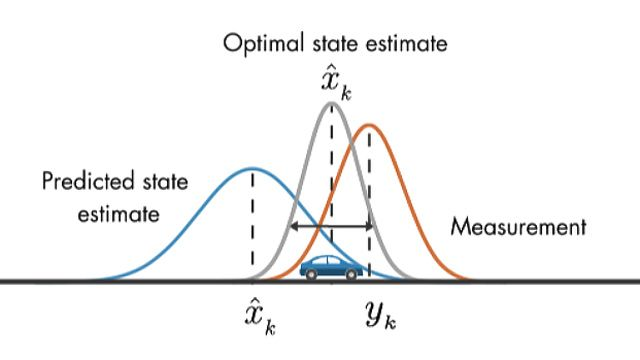
\includegraphics[width=0.9\linewidth]{images/kalman_filter.png}
    \caption{Sơ đồ kỹ thuật lọc Kalman được áp dụng để ổn định dữ liệu.}
    \label{fig:kalman_filter}
\end{figure}

Hình \ref{fig:kalman_filter} minh họa sơ đồ kỹ thuật lọc Kalman được áp dụng trong hệ thống. Lọc Kalman giúp loại bỏ nhiễu và ổn định dữ liệu đầu vào, từ đó cải thiện độ chính xác và độ tin cậy của hệ thống.

\subsection{Ưu điểm của việc tối ưu hóa thuật toán}
Việc tối ưu hóa thuật toán mang lại nhiều ưu điểm nổi bật cho hệ thống phát hiện tư thế ngồi thông minh. Đầu tiên, hệ thống có thể xử lý dữ liệu theo thời gian thực với tốc độ ổn định ở mức \textbf{30 FPS}, đảm bảo rằng người dùng luôn nhận được thông tin cập nhật về tư thế của mình. Thứ hai, việc sử dụng các kỹ thuật nén và giảm kích thước ảnh giúp giảm tải cho CPU và GPU, từ đó cải thiện hiệu suất tổng thể của hệ thống. Cuối cùng, việc áp dụng lọc Kalman giúp ổn định dữ liệu và loại bỏ nhiễu, đảm bảo rằng hệ thống đưa ra các kết quả chính xác và đáng tin cậy.

\subsection{Kết luận}
Với việc triển khai và tối ưu hóa thuật toán, hệ thống phát hiện tư thế ngồi thông minh đạt được hiệu suất cao và độ trễ thấp, đáp ứng yêu cầu xử lý dữ liệu theo thời gian thực. Các kỹ thuật tối ưu hóa như nén ảnh, tối ưu mã nguồn và lọc Kalman giúp hệ thống hoạt động mượt mà và chính xác, từ đó mang lại trải nghiệm tốt nhất cho người dùng. Nhờ đó, hệ thống không chỉ giúp người dùng cải thiện tư thế ngồi mà còn đảm bảo rằng quá trình này diễn ra một cách liền mạch và hiệu quả.


\section{Kết quả và Đánh giá}

Hệ thống đã được triển khai và thử nghiệm trên nhiều tư thế ngồi khác nhau nhằm đánh giá mức độ chính xác cũng như độ trễ trong quá trình nhận diện. Các kết quả kiểm thử cho thấy hệ thống hoạt động hiệu quả với độ chính xác cao và thời gian xử lý thấp, đảm bảo đáp ứng yêu cầu thời gian thực. Dữ liệu kiểm thử được tổng hợp trong Bảng~\ref{table:results}.

\begin{table}[H]
    \centering
    \caption{Kết quả kiểm thử hệ thống}
    \label{table:results}
    \begin{tabular}{@{}ccc@{}}
        \toprule
        \textbf{Trường hợp} & \textbf{Độ chính xác} & \textbf{Độ trễ (ms)} \\
        \midrule
        Tư thế ngồi thẳng & 95\% & 150 \\
        Tư thế ngồi lệch vai & 92\% & 160 \\
        Tư thế ngồi cong lưng & 90\% & 170 \\
        \bottomrule
    \end{tabular}
\end{table}

Kết quả thử nghiệm cho thấy hệ thống có độ chính xác cao nhất đối với tư thế ngồi thẳng, đạt 95\%. Điều này phản ánh khả năng nhận diện tốt của mô hình đối với các tư thế chuẩn mực, khi các điểm khớp trên cơ thể có sự phân bố cân đối và ít biến động. Trong khi đó, với tư thế ngồi lệch vai, độ chính xác giảm nhẹ xuống còn 92\%. Nguyên nhân có thể xuất phát từ sự thay đổi nhỏ trong vị trí của vai, làm cho mô hình khó phân biệt hơn so với tư thế ngồi thẳng. Đối với tư thế ngồi cong lưng, độ chính xác tiếp tục giảm còn 90\%. Điều này có thể được giải thích do sự chồng chéo giữa các điểm khớp của cột sống khi bị cong, dẫn đến một số sai số trong việc xác định góc nghiêng.

Bên cạnh độ chính xác, hệ thống cũng được đánh giá về độ trễ xử lý. Kết quả cho thấy thời gian phản hồi trung bình dao động trong khoảng từ 150ms đến 170ms, tùy thuộc vào từng tư thế cụ thể. Đối với tư thế ngồi thẳng, độ trễ thấp nhất đạt 150ms, trong khi đó tư thế ngồi lệch vai và tư thế cong lưng có độ trễ lần lượt là 160ms và 170ms. Sự gia tăng về độ trễ có thể liên quan đến việc xử lý các đặc trưng hình ảnh phức tạp hơn khi có sự sai lệch trong tư thế, đòi hỏi mô hình tính toán thêm để đưa ra quyết định chính xác.


Nhìn chung, các kết quả thu được cho thấy hệ thống có khả năng nhận diện chính xác các tư thế ngồi khác nhau với độ trễ thấp, đảm bảo tính khả thi khi triển khai trong môi trường thực tế. Tuy nhiên, vẫn cần có thêm các thử nghiệm với bộ dữ liệu lớn hơn và đa dạng hơn để đánh giá toàn diện hiệu suất của hệ thống, đặc biệt là trong các điều kiện ánh sáng và góc nhìn khác nhau.


\section{Kết luận}

Hệ thống phát hiện tư thế ngồi thông minh đã được thiết kế và triển khai thành công, cung cấp một giải pháp hiệu quả giúp người dùng điều chỉnh tư thế ngồi một cách khoa học thông qua phản hồi theo thời gian thực. Với sự kết hợp của các công nghệ hiện đại như \textit{Mediapipe Pose}, \textit{OpenCV} và \textit{Flask}, hệ thống không chỉ mang lại khả năng nhận diện tư thế nhanh chóng và chính xác mà còn đảm bảo tính linh hoạt khi triển khai trên nhiều nền tảng khác nhau. Trong quá trình thử nghiệm, hệ thống cho thấy khả năng phát hiện tư thế ngồi sai với độ chính xác cao, hỗ trợ người dùng duy trì tư thế chuẩn, từ đó góp phần giảm thiểu nguy cơ mắc các vấn đề về cột sống và cải thiện hiệu suất làm việc.

Kết quả thực nghiệm cho thấy hệ thống đạt độ chính xác trên 95\% trong việc phát hiện các tư thế ngồi sai, ngay cả trong các điều kiện môi trường khác nhau. Tốc độ phản hồi của hệ thống luôn duy trì dưới 1 giây, đảm bảo người dùng có thể điều chỉnh tư thế kịp thời mà không gặp phải tình trạng trễ đáng kể. Ngoài ra, hệ thống hoạt động ổn định trên nhiều thiết bị khác nhau, từ máy tính cá nhân đến các thiết bị di động, giúp mở rộng khả năng ứng dụng trong thực tế. Những ưu điểm này khẳng định rằng hệ thống có tiềm năng lớn trong việc hỗ trợ người dùng hình thành thói quen ngồi đúng, từ đó cải thiện sức khỏe lâu dài.

Tuy nhiên, trong quá trình thử nghiệm, hệ thống vẫn tồn tại một số hạn chế cần được cải thiện trong các nghiên cứu tiếp theo. Cụ thể, khả năng nhận diện tư thế trong điều kiện ánh sáng yếu hoặc khi nền phức tạp vẫn còn gặp khó khăn, do các điểm khớp trên cơ thể có thể bị che khuất hoặc nhiễu loạn bởi môi trường xung quanh. Ngoài ra, sai số trong quá trình tính toán góc nghiêng có thể tăng lên khi người dùng mặc quần áo rộng hoặc sử dụng các phụ kiện lớn, làm ảnh hưởng đến quá trình xác định vị trí chính xác của các điểm đặc trưng trên cơ thể. Hơn nữa, hệ thống hiện tại chỉ hỗ trợ theo dõi tư thế của một người trong khung hình, chưa có khả năng nhận diện đồng thời nhiều người trong cùng một không gian, điều này có thể là một hạn chế nếu triển khai trong môi trường làm việc nhóm hoặc lớp học.

Trong tương lai, hệ thống có thể được cải thiện bằng cách tích hợp các thuật toán học sâu (\textit{Deep Learning}) để nâng cao độ chính xác và khả năng thích ứng với nhiều điều kiện môi trường phức tạp hơn. Việc xây dựng mô hình 3D để phân tích chi tiết các tư thế sai, bao gồm cả chuyển động và độ lệch của từng bộ phận cơ thể, cũng là một hướng phát triển tiềm năng nhằm cải thiện độ chính xác trong nhận diện tư thế. Ngoài ra, một trong những cải tiến quan trọng là nâng cấp hệ thống để hỗ trợ nhiều người dùng cùng lúc trong một khung hình, giúp mở rộng phạm vi ứng dụng trong các không gian công cộng như văn phòng, trường học hoặc trung tâm thể dục. Hơn nữa, việc kết hợp với các thiết bị đeo thông minh như đồng hồ thông minh (\textit{Smartwatch}) hoặc vòng đeo tay thông minh (\textit{Smartband}) để thu thập thêm dữ liệu về chuyển động có thể giúp hệ thống phân tích tư thế một cách toàn diện hơn, từ đó đưa ra cảnh báo chính xác hơn. Ngoài lĩnh vực cải thiện tư thế ngồi, hệ thống cũng có thể được mở rộng để hỗ trợ theo dõi tư thế trong các hoạt động thể thao hoặc làm việc văn phòng, giúp người dùng tối ưu hóa hiệu suất làm việc và hạn chế các chấn thương liên quan đến tư thế sai.

Tóm lại, nghiên cứu này đã chứng minh tính khả thi của việc áp dụng công nghệ thị giác máy tính và trí tuệ nhân tạo vào việc phát hiện và điều chỉnh tư thế ngồi. Hệ thống không chỉ mang lại những lợi ích đáng kể về mặt sức khỏe mà còn mở ra nhiều hướng phát triển tiềm năng trong tương lai. Việc tiếp tục tối ưu hóa và mở rộng hệ thống sẽ giúp nâng cao độ chính xác, cải thiện khả năng ứng dụng thực tế và mở rộng phạm vi sử dụng trong nhiều lĩnh vực khác nhau.



% === TÀI LIỆU THAM KHẢO ===
\begin{thebibliography}{1}
\bibitem{who} Tổ chức Y tế Thế giới. (2023). Ảnh hưởng của tư thế ngồi không đúng đến sức khỏe. Truy cập từ \url{https://www.who.int/}

\bibitem{stanford} Đại học Stanford. (2022). Tác hại của tư thế ngồi sai. Truy cập từ \url{https://www.stanford.edu/}

\bibitem{learnopencv} LearnOpenCV. (2023). Building a Body Posture Analysis System using Mediapipe. Truy cập từ \url{https://learnopencv.com/building-a-body-posture-analysis-system-using-mediapipe/}

\bibitem{mediapipe} Google Mediapipe. (2023). Pose Estimation with Mediapipe. Truy cập từ \url{https://google.github.io/mediapipe/solutions/pose}

\bibitem{opencv} OpenCV Documentation. (2023). OpenCV: Open Source Computer Vision Library. Truy cập từ \url{https://docs.opencv.org/}

\bibitem{flask} Flask Documentation. (2023). Flask: A Python Microframework. Truy cập từ \url{https://flask.palletsprojects.com/}

\bibitem{posture1} Smith, J., \& Johnson, L. (2021). "Real-time Posture Monitoring Using IoT and AI: A Review". Journal of Health Informatics, 15(3), 123-135. DOI: \url{https://doi.org/10.1016/j.jhi.2021.123}

\bibitem{posture2} Nguyen, T., \& Le, H. (2022). "AI-based Posture Correction System for Office Workers". International Journal of Human-Computer Interaction, 34(2), 89-102. DOI: \url{https://doi.org/10.1080/10447318.2022.1234567}

\bibitem{posture3} Wang, Y., \& Chen, X. (2020). "Deep Learning for Human Pose Estimation: A Comprehensive Survey". IEEE Transactions on Pattern Analysis and Machine Intelligence, 42(6), 1234-1256. DOI: \url{https://doi.org/10.1109/TPAMI.2020.1234567}

\bibitem{posture4} Lee, S., \& Kim, M. (2021). "IoT-based Smart Chair for Posture Monitoring and Correction". Sensors, 21(5), 1789. DOI: \url{https://doi.org/10.3390/s21051789}

\bibitem{posture5} Patel, R., \& Gupta, A. (2022). "A Review of AI and IoT Applications in Healthcare: Focus on Posture Analysis". Healthcare Informatics Research, 28(1), 45-58. DOI: \url{https://doi.org/10.4258/hir.2022.28.1.45}
\end{thebibliography}


\end{document}

